\documentclass{article} % For LaTeX2e
\usepackage{iclr2025_conference,times}
\usepackage[T1]{fontenc}
\usepackage[utf8]{inputenc}
\usepackage{graphicx}
\usepackage{amsmath,amssymb,amsfonts}  % Enhanced math support
\usepackage{booktabs}                   % Better tables
\usepackage{multirow}                   % Multi-row cells in tables
\usepackage{tabularx}                   % Tables with adjustable columns
\usepackage{xcolor}                     % Color support
\usepackage{microtype}                  % Better typography
\usepackage{subcaption}                 % Subfigures and subcaptions
\usepackage{algorithm2e}                % Algorithm formatting
\usepackage{tikz}                       % Drawing and diagrams
\usepackage{wrapfig}                    % Wrap text around figures
\usepackage{makecell}                   % Cell formatting with line breaks

% Optional math commands from https://github.com/goodfeli/dlbook_notation.
\input{math_commands.tex}

\usepackage{hyperref}
\usepackage{url}
\usepackage{cleveref}                   % Better cross-referencing (must be after hyperref)
\usepackage{listings}                   % Code/prompt listings in boxes
\lstset{basicstyle=\ttfamily\small, frame=single, breaklines=true, columns=fullflexible, literate={<}{{\textless}}1 {>}{{\textgreater}}1}

% Define theorem-like environments
\usepackage{amsthm}
\theoremstyle{definition}
\newtheorem{definition}{Definition}[section]


\title{Can Models refuse questions they don't know? \\ Measuring Knowledge-aware Refusal in LLMs}

% Authors must not appear in the submitted version. They should be hidden
% as long as the \iclrfinalcopy macro remains commented out below.
% Non-anonymous submissions will be rejected without review.

\author{Antiquus S.~Hippocampus, Natalia Cerebro \& Amelie P. Amygdale \thanks{ Use footnote for providing further information
about author (webpage, alternative address)---\emph{not} for acknowledging
funding agencies.  Funding acknowledgements go at the end of the paper.} \\
Department of Computer Science\\
Cranberry-Lemon University\\
Pittsburgh, PA 15213, USA \\
\texttt{\{hippo,brain,jen\}@cs.cranberry-lemon.edu} \\
\And
Ji Q. Ren \& Yevgeny LeNet \\
Department of Computational Neuroscience \\
University of the Witwatersrand \\
Joburg, South Africa \\
\texttt{\{robot,net\}@wits.ac.za} \\
\AND
Coauthor \\
Affiliation \\
Address \\
\texttt{email}
}

% The \author macro works with any number of authors. There are two commands
% used to separate the names and addresses of multiple authors: \And and \AND.
%
% Using \And between authors leaves it to \LaTeX{} to determine where to break
% the lines. Using \AND forces a linebreak at that point. So, if \LaTeX{}
% puts 3 of 4 authors names on the first line, and the last on the second
% line, try using \AND instead of \And before the third author name.

\newcommand{\fix}{\marginpar{FIX}}
\newcommand{\new}{\marginpar{NEW}}
\newcommand{\cm}[1]{\textcolor{red}{#1}}
% \newcommand{\cm}[1]{}
\newcommand{\bt}[1]{\textcolor{blue}{#1}}

%\iclrfinalcopy % Uncomment for camera-ready version, but NOT for submission.
\begin{document}


\maketitle

\begin{abstract}
Large Language Models (LLMs) should refuse to answer questions beyond their knowledge, which is a crucial ability for LLMs to be reliable. 
However, existing metrics face three challenges in quantifying this ability: 
\textbf{(1) inaccurate:} yielding inconsistent and biased scores; 
\textbf{(2) complex:} requiring heavy calibration processes; 
and \textbf{(3) indirect:} measuring auxiliary models rather than refusal behavior. 
In this work, we propose a new metric called \emph{Refusal Index (RI)} to measure how accurately LLMs refuse questions they do not know. 
We define RI as Spearman's rank correlation between the refusal probability and the error probability. 
To calculate RI, we propose a simple and principled two-pass evaluation that estimates RI from refusal rates in two evaluation runs. 
Experiments across 16 models and 5 datasets show that RI quantifies a model's ability to make accurate knowledge-aware refusals. Unlike existing metrics, RI remains consistent when models exhibit different refusal rates.
RI addresses an important but previously untested aspect of LLM factual evaluation. 
Our observations reveal a blind spot in LLM factual evaluations: 
while LLMs are achieving higher accuracy on factual evaluations, they are not always improving their refusal behavior. 
This finding highlights the need to complement traditional metrics with the Refusal Index for comprehensive factual evaluation.

\end{abstract}

\section{Introduction}
\label{sec:intro}

Large Language Models (LLMs) are increasingly used for knowledge-intensive tasks, such as long-term reasoning~\citep{chen2025reasoningerasurveylong} and specialized expert domains~\citep{wang2025capabilitiesgpt5multimodalmedical,gu2024legalagentbench,mahdavi2025brains}. 
Despite these capabilities, LLMs are often poorly calibrated, confidently providing incorrect answers~\citep{Huang_2025}. 
An intuitive solution is to enable models to refuse questions beyond their knowledge~\citep{yin2023large}. 
Recent work has explored and strengthened this ability by inducing more accurate refusals with prompting~\citep{cheng2024aiassistantsknowdont, kadavathLanguageModelsMostly2022} or fine-tuning~\citep{zhang2024rtuninginstructinglargelanguage, kapoor2024large}. However, there lacks a reliable metric to quantify this ability.

In this paper, we refer this ability of \emph{how well LLMs refuse questions they don't know} as \emph{knowledge-aware refusals}.
Knowledge-aware refusal assesses refusal in two aspects: how well a model refuses questions beyond its knowledge (avoiding \emph{overconfidence}) and how well it avoids refusing questions it would answer correctly (avoiding \emph{over-refusing}). 
% Specifically, we aim to measure the correlation between refusal decisions and the error probability. 
We find that existing metrics struggle to capture this important property due to three limitations:

\begin{figure}[t]
    \centering
    
\includegraphics[width=0.95\linewidth]{Figures/RefusalIndex-Illustration.pdf}
    \caption{Illustration of Refusal Index (RI). Refusal Index quantifies a model's internal capability to refuse questions beyond its knowledge, by measuring the correlation between refusal decisions and the answer incorrectness. Left: Refusal Index models how correct answer rate drops with increasing refusal rate. Right: Empirical accuracies of the same model with different refusal rates align with the Refusal Index. }
    \label{fig:refusal_index_illustration}
\end{figure}

The first limitation is that existing metrics are \textbf{(1) inaccurate} for the purpose of measuring the self-knowledge.
Prior factuality evaluations~\citep{bangHalluLensLLMHallucination2025,wei2024measuringshortformfactualitylarge, zhang2024rtuninginstructinglargelanguage} report combinations of \emph{correct answer rate} and \emph{refusal rate} to quantify accuracy of LLM refusals.
These combinations measure whether a model generates more correct answers while refusing more questions it does not know at the same time.
We find that combinations of the correct answer rates and refusal rates is not sufficient to measure the self-knowledge accurately, especially when models exhibit different refusal rates. 
This inaccuracy is evidenced in  \S\ref{sec:validating_latent_uncertainty_model}: If the same model exhibits different refusal rates, these combinations return varying and biased scores.

A more rigorous approach is to measure the self-knowledge with \emph{calibration error}~\citep{guo2017calibration}, but it is \textbf{(2) complex} and \textbf{(3) indirect}. 
Calibration error measures the difference between prediction probabilities and the probability of being correct, which is close to our goal. 
However, calibration errors are computationally \textbf{complex}. 
As prediction probabilities are not directly accessible from LLM answers, these metrics require a calibration process to generate prediction probabilities from model outputs~\citep{kadavathLanguageModelsMostly2022}. 
This process can be expensive, with some methods requiring resampling up to 100 times~\citep{wei2024measuringshortformfactualitylarge} or fine-tuning language models~\citep{ulmer-etal-2024-calibrating}. 
Beyond complexity, calibration error is an \textbf{indirect} estimate: it measures the accuracy of the calibration process, which does not directly translate to the accuracy of an LLM’s refusal decisions.

In this work, we design a metric called \emph{Refusal Index (RI)} to address the weaknesses of previous metrics. 
We first formally define the Refusal Index as the Spearman's correlation between refusal probabilities and error probabilities (\S\ref{sec:refusal_index_method}). 
We then introduce a principled two-pass evaluation to estimate RI directly from refusal rates. 
Specifically, we first evaluate a model on a question-answering dataset, collecting correct answer rates and a set of refused questions. 
Then, we run a second evaluation pass to regenerate answers for questions refused in the first pass. 
Finally, we estimate the Refusal Index with correct answer rates and refusal rates from the two evaluation passes. 

We measure RI across 16 models on 5 datasets and perform extensive analyses. 
In \S\ref{sec:validating_latent_uncertainty_model}, we first demonstrate how RI quantifies the capability of models to refuse questions they don't know. 
RI parameterizes an accuracy-refusal curve describing how correct answer rate drops as the refusal rate increases. 
The curve’s convexity uniquely captures a model’s ability to reduce false refusals. We illustrate the curve in \Figref{fig:refusal_index_illustration}.
Then, to empirically validate RI, we first verify that the two-pass evaluation returns consistent RI scores on the same model with different refusal rates, aligning with the accuracy-refusal curve. 
We then demonstrate that the RI scores from the two-pass evaluation correlate strongly with established calibration methods such as AUROC with resampling ~\citep{kadavathLanguageModelsMostly2022,ulmerCalibratingLargeLanguage2024}.

Refusal Index fills an important but overlooked gap in LLM factual evaluation. 
In \S\ref{sec:discussion}, our observations reveal that (1) RI identifies models that are factually accurate but make poor refusal decisions on questions outside their knowledge, and (2) while newer models show across-the-board improvements on factual tasks, their Refusal Index does not always improve. 
This finding highlights the need to complement traditional metrics with the Refusal Index for comprehensive factual evaluation.

\section{Refusal Index}
\label{sec:refusal_index_method}

% We begin by defining the scope and objective of our research. When evaluating calibration, we want to measure whether, higher confidence in model answers leads to a higher accuracy. More precisely, whether the model's output probability aligns with the actual probability of being correct. However, evaluating either probability or correctness for arbitrary text outputs remains an open problem, as ground truth can be subjective, non-deterministic, or unavailable.

\paragraph{Problem.} When designing a pragmatic metric to measure LLM's ability to refuse questions beyond it knowledge, we face some challenges.
First, refusals in LLMs is not fully determined by its self-knowledge, because refusal decision may be affected by model preference, risk of the questions, or simply instructions. 
This precludes simply counting refusal rates for evaluating self-knowledge. 
For example, if we measure refusal rate on a set of unanswerable questions, model designed to have higher refusal rate can easily reach higher score. 
On the other hand, we want to measure refusal behavior directly without using calibrators like verbalized confidence~\citep{xiong2023can} or output from linear probes to replace refusals. 
Performance of calibrators may not reflect model self-knowledge with refusal. 
Therefore, a good metric of refusal-based self-knowledge shoud have following properties: (1) quantify model self-knowledge with refusal (2) keep consistent even when model exhibits different refusal rates. (3) derived directly from answers of blackbox LLM.

\paragraph{Notations.} Following recent factuality evaluations such as SimpleQA~\citep{wei2024measuringshortformfactualitylarge}, we focus on factual questions where model outputs can be classified as either correct or incorrect. 
To avoid hallucinated responses, models are allowed to abstain by producing outputs such as \emph{``I don't have enough information...''} to avoid giving hallucinated responses.
More formally, we denote the LLM as $f_{\text{LM}}: \mathcal{X} \rightarrow \mathcal{Y} \cup \{\bot\}$, where $x \in \mathcal{X}$ represents the input question, $y \in \mathcal{Y}$ represents the output answer, and $\bot$ denotes abstention (refusal). 
For the $i$-th question $x_i$ with ground truth $y_i$ in dataset $D$, we define the following indicators: $W_i = \mathbf{1}\{f_{\text{LM}}(x_i) \neq y_i\}$ for incorrect output and $R_i = \mathbf{1}\{f_{\text{LM}}(x_i) = \bot\}$ for refusal responses. 
We define the question difficulty as $w_i = P(f_{\text{LM}}(x_i) \neq y_i)$ as the probability of error, and $r_i = P(f_{\text{LM}}(x_i) = \bot)$ as the probability of refusal. 
We treat $w_i$ and $r_i$ as unobservable variables on $[0, 1]$. 

\paragraph{Defining Refusal Index.}
Conceptually, with better self-knowledge, the model should have a higher probability of refusal when the question becomes more difficult. 
We propose to measure this ability with \emph{Refusal Index}. 
Inspired by rank-based calibration metrics like AUROC~\citep{NiculescuMizil2005PredictingGP}, we define the refusal index to correlate refusal probabilities with error probabilities:

\begin{definition}[Refusal Index]
The Refusal Index is the Spearman's rank-correlation between the model's refusing probability $r_i$ and the error probability $w_i$.

\begin{equation}
   \text{Refusal Index} = \rho_S  = \text{Corr}(\text{Rank}(r_i), \text{Rank}(w_i))
\end{equation}

\end{definition}

We use $\rho_S$ to denote the Refusal Index for notational simplicity. 
To understand the intuition behind the definition, we say a model is \emph{perfect-refusal-self-aware} when the probability of refusal is monotonically increasing with error probability, resulting the model being more likely to refuse when the question becomes more difficult.

\begin{equation}
P(f_{\text{LM}}(x_i) = \bot) \leq P(f_{\text{LM}}(x_j) = \bot) \iff w_i \leq d_j
\label{eq:refusal_perfect_calibrated}
\end{equation}

Note that this differs from error-based calibration metrics like Expected Calibration Error (ECE), which quantify the absolute discrepancy between $r_i$ and $w_i$. 
In contrast, our approach evaluates only the rank discrepancy between $r_i$ and $w_i$.
We define the RI as a discrimination property because it captures a more fundamental aspect of refusal-based self-knowledge. 
While overall refusal rates can be adjusted through input context or model preference learning, discriminative capability is more robust and consistent. 
In the following sections, we introduce how to estimate the Refusal Index with two evaluation passes (\S\ref{sec:two_pass_evaluation}).

\subsection{Two-Pass Evaluation}
\label{sec:two_pass_evaluation}

The naive way to measure RI is to acquire the probability of refusal $P(f_{\text{LM}}(x_i) = \bot)$ on questions of varying error probabilities. 
However, refusal probability is not directly accessible from a single evaluation run. 
To infer the correlation between two latent continuous variables from binary observations, we propose the a principled two-pass evaluation process. 
The two-pass evaluation models the refusal decision with two components: (1) treat refusal and correctness as thresholding of their respective probabilities; and (2) model their joint distribution with a Guassian copula. 


\paragraph{Formulating the Joint Distribution.} In order to estimate $\rho_S$ from the joint distribution of the refusal and error probabilities, we use a Gaussian–copula model for the joint distribution with the correlation $\rho$:

\begin{equation}
C(u,v) = \Phi_\rho\!\big(\Phi^{-1}(u), \Phi^{-1}(v)\big)
\end{equation}

where $u = F_r(r_i)$ and $v = F_e(w_i)$ are the marginal CDFs, $\Phi^{-1}$ is the standard normal quantile function, and $\Phi_\rho$ is the bivariate standard normal CDF with correlation $\rho$. 
The $\Phi_\rho$ depends only on the rank correlation, decoupled from marginal distributions of the two probabilities. 
In what follows we avoid modeling $F_r$ and $F_e$ directly and estimate $\rho$ from $R_i$ and $W_i$ via maximum likelihood. 
We can then compute $\rho_S$ from $\rho$ using the relationship $\rho_S = \frac{6}{\pi}\arcsin\!\left(\frac{\rho}{2}\right)$.

To estimate $\rho$, we need to observe two binary coarsenings for each sample: $R_i$ for the refusal probability $r_i$ and $W_i$ for the error probability $w_i$. 
To this end, we propose a two-evaluation pass that evaluate the model on the same dataset twice: first pass to observe refusal $R_i$ and second pass to observe correctness $W_i$. 
In the first pass, we use a standard setup to allow model answer or refuse each question, where we classify responses into correct, incorrect, or refused. 
In the second pass, we update the system prompt to remove the content related to the abstention policy and only prompt the model to answer questions. We provide prompt details in \S\ref{app:system_prompts} 
We perform the second pass only on the subset of questions that were refused in the first pass, collecting the correctness indicators $W'_i$ for all refused questions ($R_i = 1$).

\begin{wrapfigure}{r}{0.5\textwidth}
    \centering
    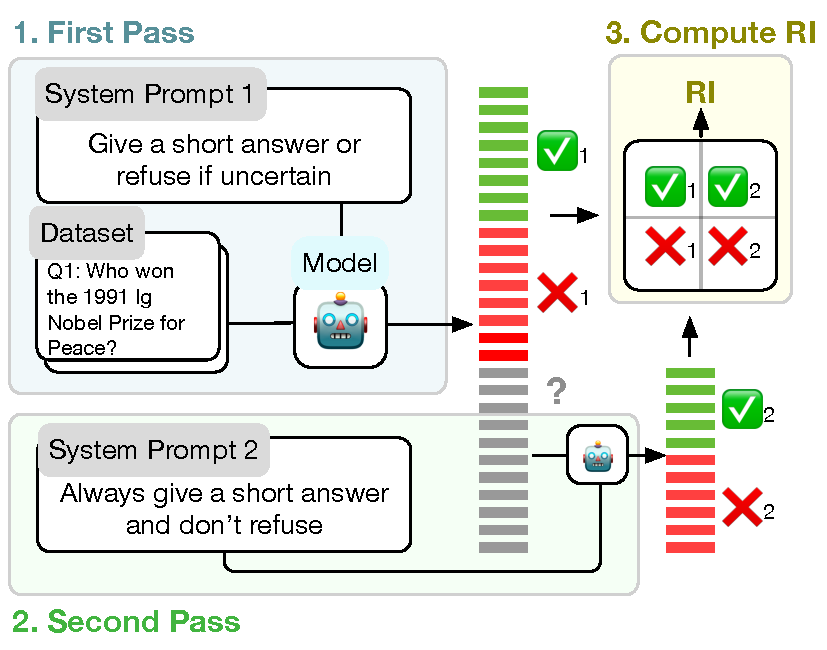
\includegraphics[width=0.45\textwidth]{Figures/two-pass.pdf}
    \caption{Illustration of two-pass evaluation process.}
    \label{fig:two_pass_evaluation}
\end{wrapfigure}

\paragraph{Estimating Refusal Index.} We defined the aggregated correctness indicator $\hat{W}_i = \mathbf{1}\{W'_i = 1\text{ if } R_i = 1 \text{ else } W_i\}$ as the correctness indicator when the model answered the question. 
Let the empirical refusal rate be $r=\sum_{i=1}^{|D|} R_i/|D|$ and the incorrect rate be $\mu = \sum_{i=1}^{|D|} \hat{W}_i/|D|$. 
Under the latent uncertainty model, the pair $(R,\hat{W})$ arises by thresholding a bivariate standard normal vector $(Z_R,Z_W)$ with correlation $\rho$ at

$$
\tau_R=\Phi^{-1}(1-r), \qquad \tau_W=\Phi^{-1}(1-\mu).
$$

Let $n_{ab}$ be the counts of $(R=a, \hat{W}=b)$ for $a,b\in\{0,1\}$. The cell probabilities are

$$
\begin{aligned}
p_{11}(\rho) &= \bar\Phi_2\!\big(\tau_R,\tau_W;\rho\big) \;=\; P(Z_R>\tau_R, Z_W>\tau_W),\\
p_{10}(\rho) &= r - p_{11}(\rho),\qquad
p_{01}(\rho) \;=\; \mu - p_{11}(\rho),\\
p_{00}(\rho) &= 1 - r - \mu + p_{11}(\rho),
\end{aligned}
$$

We estimate $\hat\rho$ by maximizing the multinomial log-likelihood, which are then used to compute $\rho_S$:
\begin{align}
\hat\rho = \argmax_{\rho \in (-1,1)} \ell(\rho), \quad \text{where} \quad \ell(\rho) = \sum_{a,b\in\{0,1\}} n_{ab} \log p_{ab}(\rho).
\label{eq:ri-estimation}
\end{align}

\section{Experiments \& Results}
\label{sec:experiments}

\subsection{Experimental Setup}
\label{sec:experimental_setup}

\paragraph{Models} We evaluate RI on 16 open-source and proprietary models, covering different model families, sizes and release dates. 
Open-source models include \emph{Gemma-3-12B}~\citep{gemma3_2025}, \emph{Qwen3-32B/235B}~\citep{qwen3_2025} in both think and no-think mode, \emph{Qwen2.5-72B-Instruct}~\citep{qwen2_5_2024}, \emph{Llama 3.1 70B} \citep{llama3_2024}, \emph{Mistral-Large-Instruct-2411}~\citep{mistral_large_2_2024}, \emph{GLM-4.5 and GLM-4.5-Air}\citep{glm45_2025} and \emph{DeepSeek-V3-0324}~\citep{deepseek_v3_2024}. 
For proprietary models, we use \emph{Claude 3.5 haiku} \citep{claude35_2024}, \emph{Claude Sonnet 4} \citep{claude4_2025}, \emph{GPT4.1} and \emph{GPT4.1 mini} \citep{gpt41_2025} and \emph{Gemini 2.5 Flash} and \emph{Gemini 2.5 Flash Lite} \citep{gemini25_2025}. 
We use temperature=0.7 , top-p=0.95 for all models.

\paragraph{Datasets} We evaluate RI on 3 scenarios: factual question answering, extrinsic hallucination detection (hallucination from training data), and intrinsic hallucination detection (hallucination from context), which all require the model's ability to make proper, self-aware refusals. 
For factual question answering, we use SimpleQA \citep{wei2024measuringshortformfactualitylarge}. 
SimpleQA contains verifiable, atomic factual questions that is even challenge for frontier LLMs. 
For extrinsic hallucination detection, we use PreciseWikiQA \citep{bangHalluLensLLMHallucination2025}. 
PreciseWikiQA is a dynamically generated question answering dataset from snippets of wikipedia. 
It tests if model hallucinate its training data, given the knowledge (wikipedia) is assumed to be included in training data. 
We follow the \citet{bangHalluLensLLMHallucination2025} to generate 2000 questions for evaluation. 
Finally, for intrinsic hallucination detection, we use the 3 datasets from FaithEval \citep{ming2025faithevallanguagemodelstay}. 
FaithEval tests if the model can faithfully recall the information with a noisy context. 
We use all 3 datasets from FaithEval. 
However, as the \texttt{Unanswerable} and \texttt{Inconsistency} subset do not have ground truth, which RI needs for correct answer rate, we create a 1:1 mixed dataset of PreciseWikiQA and FaithEval to report RI.

\paragraph{Baseline Metrics} We compare RI with 5 metrics from SimpleQA and HalluLens that are used for measuring refusal-based self-knowledge, shown in Table~\ref{tab:baseline_metrics}, including Correct Answer Rate, Refusal Rate, Correct given Attempted (C/A), F-score, and Weighted Score. 
We pick $p=0.5$ for the Weighted Score. 
To produce all metrics, we follow SimpleQA to classify model output into either (In) Correct, (2) Incorrect, or (3) Not Attempted (refusal). 
Additionally, we further compare RI with calibration metrics AUROC with P(Answering) as an uncertainty estimation method. 
We follow the \citet{wei2024measuringshortformfactualitylarge} to compute P(Answering) by sampling 100 times from each question input under temperature=1 and then setting the predition probability of the question to be $1 - N_\text{refusal}/N$, where $N_\text{refusal}$ is the number of refusal answers. 
The AUROC score between P(Answering) and correctness labels can be approximately served as the golden reference for Refusal Index. 


\begin{table}[t]
    \centering
    \footnotesize
    \caption{Baseline factuality metrics used for comparison. $c$ and $r$ denotes correct answer rate and refusal rate, respectively.}
    \begin{tabularx}{\textwidth}{l X l}
        \toprule
        \textbf{Metric} & \textbf{Formula} & \textbf{Definition} \\
        \midrule
        Correct Answer Rate & $c$ & Proportion of correct answers \\
        Refusal Rate & $r$ & Proportion of refusal answers \\
        Correct given Attempted (C/A) & $c/(1 - r)$ & Correct answer rate among answered questions \\
        F-score & $2c/(2 - r)$ & Harmonic mean of Correct Answer Rate and C/A \\
        Weighted Score & $c - p(1-r)$ & Weighted difference of $c$ and $r$ \\
        \midrule
        Refusal Index & Eq. \ref{eq:ri-estimation} & Correlation between refusal decision and incorrectness \\
        \bottomrule
    \end{tabularx}
    \label{tab:baseline_metrics}
\end{table}

\paragraph{Adjusting Refusal Rates} We measure how the Refusal Index changes when the model exhibit different refusal rates. 
To this end, we use different system prompts to instruct the model to be more proactive or cautious in answering questions. 
Models are prompted to have different refusal tendencies without degrading its decision quality. 
Specifically, other than the default system prompt that make model answer all questions in the second pass, we use 4 different system prompts to evaluate each model with different refusal rates in the first pass. The details of the system prompts are shown in \S\ref{app:system_prompts}.


\subsection{Refusal Rate Stability Analysis}
\label{sec:validating_latent_uncertainty_model}


\begin{table*}[t]
    \centering
    \small
    \caption{Score stability across different refusal rates. We run evaluation with different refusal tendencies on SimpleQA for each model. $\Delta_{\text{Metric}}$ denotes the normalized difference between most-refusal and least-refusal runs. We use $p=0.2$ for the Weighted metric. Lower is better.}
    \label{tab:qwen25_simpleqa_prompt_strategies}
    \begin{tabularx}{\textwidth}{>{\raggedright\arraybackslash}p{0.12\textwidth} >{\raggedright\arraybackslash}p{0.15\textwidth} *{6}{>{\centering\arraybackslash}X}}
        \toprule
        \textbf{Type} & \textbf{Model} & \textbf{$\Delta_{\text{Accuracy}}$} & \textbf{$\Delta_{\text{Refusal}}$} & \textbf{$\Delta_{\text{C/A}}$} & \textbf{$\Delta_{\text{F-score}}$} & \textbf{$\Delta_{\text{Weighted}}$} & \textbf{$\Delta_{\text{RI}}$} \\
        \midrule
        \multirow{5}{*}{\makecell{Normalized \\ Difference}} & Mistral-123B & $-0.40$ & $+0.93$ & $+0.37$ & $-0.16$ & $-0.83$ & $\mathbf{+0.06}$ \\
         & Qwen2-35B & $-0.47$ & $+0.95$ & $+0.12$ & $-0.31$ & $-0.62$ & $\mathbf{-0.19}$ \\
         & Qwen2.5-72B & $-0.84$ & $+0.43$ & $+0.50$ & $-0.60$ & $-1.32$ & $\mathbf{-0.07}$ \\
         & Qwen3-32B & $-0.96$ & $+0.54$ & $+0.48$ & $-0.71$ & $-1.42$ & $\mathbf{+0.14}$ \\
         & Average & $-0.73$ & $+0.72$ & $+0.50$ & $-0.50$ & $-1.17$ & $\mathbf{+0.08}$ \\
        \midrule
         & \textbf{Model} & \textbf{$CV_{\text{Accuracy}}$} & \textbf{$CV_{\text{Refusal}}$} & \textbf{$CV_{\text{C/A}}$} & \textbf{$CV_{\text{F-score}}$} & \textbf{$CV_{\text{Weighted}}$} & \textbf{$CV_{\text{RI}}$} \\
        \midrule
        \multirow{5}{*}{\makecell{Coefficient of \\ Variation}} & Mistral-123B & $0.16$ & $0.35$ & $0.14$ & $0.06$ & $0.31$ & $\mathbf{0.04}$ \\
         & Qwen2-35B & $0.22$ & $0.47$ & $0.06$ & $0.14$ & $0.32$ & $\mathbf{0.09}$ \\
         & Qwen2.5-72B & $0.35$ & $0.17$ & $0.19$ & $0.26$ & $0.53$ & $\mathbf{0.03}$ \\
         & Qwen3-32B & $0.35$ & $0.19$ & $0.17$ & $0.28$ & $0.51$ & $\mathbf{0.07}$ \\
         & Average & $0.29$ & $0.29$ & $0.19$ & $0.21$ & $0.46$ & $\mathbf{0.08}$ \\
        \bottomrule
    \end{tabularx}
\end{table*}


In this section we validate Refusal Index and analyze its stability across different refusal rates. 
We demonstrate that: (1) the Refusal Index conceptualizes and evaluates the model's refusal-based self-knowledge with \emph{accuracy-refusal curve}, and (2) the two-pass evaluation returns consistent RI across different refusal rates.

\paragraph{RI Measures Knowledge-aware Refusal with Accuracy-Refusal Curve}
We can use an accuracy-refusal curve to measure the accuracy of knowledge-aware refusal, which shows the correct answer rate at each refusal rate for a model on the same dataset.
While refusing more uncertain questions reduces incorrect answers, it also leads to less correct answers due to false refusals. 
By varing overall refusal tendency, each model has a trade-off between correct answers and refusal rate. 
As shown in Figure~\ref{fig:acc_rej_plot_with_contour_lines}, fixing any metric constant gives a unique iso-score curve in the accuracy–refusal plane, which describe the accuracy-refusal trade relationship assumed by the metric.

\begin{wrapfigure}{r}{0.48\textwidth}
    \centering
    \vspace{-1.5em}
    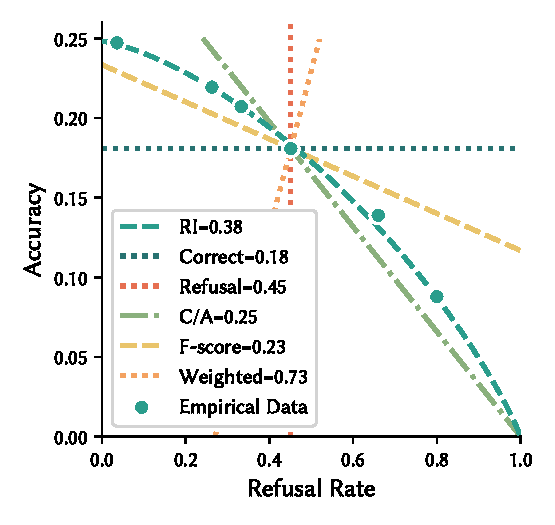
\includegraphics[width=0.48\textwidth]{Figures/acc_rej_plot_with_contour_lines.pdf}
    \caption{Comparison of factuality metrics with iso-score accuracy-refusal trade-off curves. C/A, F, and W correspond to Correct / Attempted, F-score, and Weighted score, respectively.}
    \vspace{-1em}
    \label{fig:acc_rej_plot_with_contour_lines}
\end{wrapfigure}


Compared with heuristic metrics, iso-RI curves have two desirable interpretable properties: (1) they represent sensible accuracy–refusal trade-offs matching the expected behavior of the model (see Figure~\ref{fig:refusal_index_illustration}, left). 
Different iso-RI curves yield the same maximum correct answer numbers when the refusal rate is 0 and reaching zero correct answers when the refusal rate is 1; and (2) RI is agnostic to maximum correct answer numbers and refusal rate, and it controls only the convexity of the curve, capturing how well a model preserves correct answers by reducing false refusals. 
That is, for two models with the same max correct answer numbers, the one with higher RI retains more correct answers when refusing the same fraction of questions. 
In contrast, heuristic metrics fail to capture this property, imposing approximately linear accuracy–refusal relationships at fixed scores. 
In summary, the Refusal Index does not simply reward higher accuracy or lower refusal rate, but captures the level of rank-calibration in refusal decisions, distinct from all previous metrics.

% \begin{figure}[t]
%     \centering
%     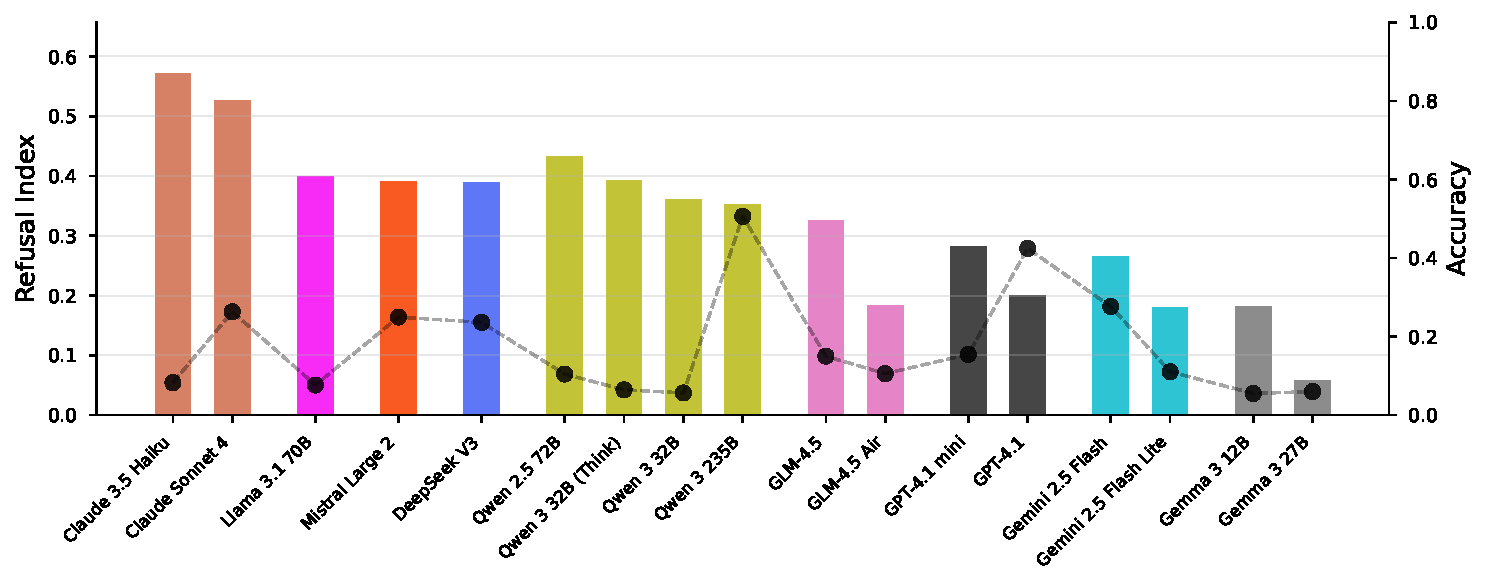
\includegraphics[width=0.95\linewidth]{Figures/simpleqa_refusal_index.pdf}
%     \caption{Evaluation results of the Refusal Index on SimpleQA. }
%     \label{fig:simpleqa_refusal_index}
% \end{figure}

\paragraph{RI remains consistent across different refusal rates.}

To empirically validate RI, we test whether the Refusal Index remains consistent across different refusal rates. 
For this, we design a set of system prompts that progressively encourage caution in answering to induce different refusal rates, and then apply them to the same model on the SimpleQA dataset. 
Our results demonstrate that RI exhibits remarkable stability across these different refusal rates, while heuristic metrics show substantial variation. 
As shown in Table~\ref{tab:qwen25_simpleqa_prompt_strategies}, RI is around 70\% lower in variability compared to heuristic metrics. 
This empirical finding suggests that prompt-induced changes in refusal rate shift the refusal probability distribution without changing the correlation between refusal probability and error probability. 
In the appendix, we provide additional validation through goodness-of-fit tests for the Gaussian copula assumption.


\subsection{Alignment with Calibration Methods}

\paragraph{RI is highly consistent with sampling-based calibration methods.}
One potential concern with RI is that although it is defined as the rank correlation between refusal probability and error probability, the two-pass evaluation may not faithfully reflect that correlation. 
To address this, we further compare RI values with AUROC with P(Answering) as an uncertainty estimation method. 
We choose AUROC with P(Answering) for fair comparison because it shares the same definition of uncertainty as RI. 
Specifically, (1) AUROC is a rank-calibration metric that only measure the discriminative ability of refusal and (2) P(Answering) is a direct and naive estimation of prediction probability of model refusals. 
While there exist other calibration metrics like ECE, Brier Score and various uncertainty estimation methods, AUROC with P(Answering) is the most direct measurement of the correlation between refusal and error.
\Figref{fig:comparison_auroc} shows the results. 
Among the evaluated metrics, RI demonstrates the strongest positive correlation with AUROC at 85\%, outperforming all other metrics.
This high agreement between RI and AUROC with P(Answering) suggests that RI accurately reflects the correlation between refusal probability and error probability.
Meanwhile, RI requires much smaller compute overhead compared to estimate P(Answering) with multiple sampling.


\begin{figure}[t]
    \centering
    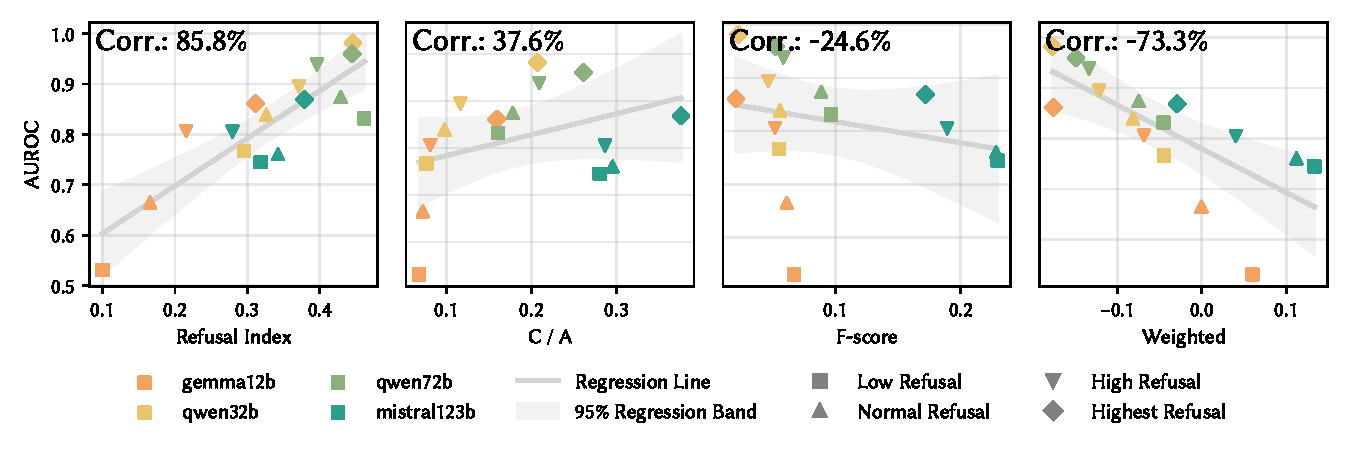
\includegraphics[width=\linewidth]{Figures/comparison_auroc_panswer.pdf}
    \caption{Correlation between factuality metrics and AUROC with P(Answering) on SimpleQA. RI shows the highest positive correlation with AUROC while being orders of magnitude cheaper to compute.}
    \label{fig:comparison_auroc}
\end{figure}

\subsection{Model Ranking Stability}

Finally, we study if the knowledge-aware refusal measured by RI is consistent across different models and datasets. 
To this end, we measure model ranking stability: does RI rank models consistently in different datasets or evaluation settings? 
Higher ranking stability suggests that a metric captures genuine, discriminative property of models. 
Specifically, we calculate Kendall's $W$ (overall ranking agreement) and Winner Entropy (top1 consistency) on all of our 8 evaluation settings (4 refusal-varying evaluation on SimpleQA + 4 hallucination benchmarks). 
Additionally, to capture the ranking stability of the correlation structure between correct answers and refusals, we want to filter out the effect from solely the correct answer rate or refusal rate. 
We make the removal by performing a isotonic regression on the correct answer rate or refusal rate across different setups for each, then remove regressed values from each metric. We calculate the Kendall's $W$ and Winner Entropy on the residual, effectively measuring parts of the metric that cannot be explained by correct answer rate or refusal rate alone.

\paragraph{RI provide stable model ranking independent of accuracy and refusal rate.} 
As shown in Table~\ref{tab:ranking_stability}, when removing the monotonic effect of correct answer rate or refusal rate, RI still shows high ranking stability, while heuristic metrics degrade to near random values. 
We can see that heuristic metrics like F-score and Weighted achieve very good ranking stability, but their Kendall's $W$ and Winner Entropy drops quickly when we remove the monotonic effect from correct answer rate or refusal rate. 
This result suggests that while heuristic metrics like F-score has high ranking stability, they are mostly explained by correct answer rate or refusal rate. 
In contrast, RI retains most of its ranking stability even after removing the effect from correct answer rate and refusal rate, indicating that it captures the intrinsic knowledge-aware refusal of models, persisting across different evaluation settings.


\begin{table}[t]
    \centering
    \small
    \caption{Ranking stability across different evaluation settings. $-\text{Correct}$ and $-\text{Refusal}$ show results after removing monotonic effects of correct answer rate and refusal rate with isotonic regression. $- \text{Both}$ removes both correctness and refusal rates with additive isotonic regression.}
    \label{tab:ranking_stability}
    \setlength{\tabcolsep}{4pt}
    \begin{tabular}{lcccccccc}
        \toprule
         & \multicolumn{4}{c}{\textbf{Kendall's W} $\uparrow$} & \multicolumn{4}{c}{\textbf{Winner Entropy} $\downarrow$} \\
        \cmidrule(lr){2-5} \cmidrule(lr){6-9}
        \textbf{Metric} & \textbf{Default} & \textbf{$- \text{Correct}$} & \textbf{$- \text{Refusal}$} & \textbf{$- \text{Both}$} & \textbf{Default} & \textbf{$- \text{Correct}$} & \textbf{$- \text{Refusal}$} & \textbf{$- \text{Both}$} \\
        \midrule
        Random Value  & 0.25 & 0.25 & 0.25 & 0.25 & 0.61 & 0.61 & 0.61 & 0.61 \\
        Correct Answer Rate & 0.87 & 0.00 & \textbf{0.48} & 0.39 & \textbf{0.00} & 1.00 & 0.48 & 1.00 \\
        Refusal Rate & 0.86 & 0.44 & 0.00 & 0.30 & 0.18 & 0.61 & 1.00 & 1.00 \\
        \midrule
        C / A    & 0.69 & \textbf{0.63} & 0.40 & 0.37 & 0.33 & 0.61 & 0.48 & 0.61 \\
        F-score  & \textbf{0.90} & 0.10 & 0.48 & 0.39 & 0.00 & \textbf{0.18} & 0.48 & 0.52 \\
        Weighted & 0.87 & 0.60 & 0.25 & 0.32 & 0.33 & 0.33 & \textbf{0.37} & 0.61 \\
        RI       & 0.47 & 0.50 & 0.35 & \textbf{0.49} & 0.47 & 0.33 & 0.61 & \textbf{0.37} \\
        \bottomrule
    \end{tabular}%
    \\
\end{table}


\section{Discussion}
\label{sec:discussion}

In previous section, we have validated the Refusal Index with its analytical model and experimental results, showing that the RI uniquely and consistently evaluates the knowledge-aware refusal ability. In this section, we provide observations into LLM factuality through the lens of Refusal Index. Our interpretable and practical method provides several new insights into model calibration that were previously obscured by heuristic metrics. 


\paragraph{Does prompting models to be more cautious mitigate miscalibration?} LLMs are notorious for their overconfidence, by default, LLMs will try to answer all questions beyond their knowledge. One will be curious if instructing models to reduce confidence helps with this problem. Our proposed Ri gives a more holistic understanding to this question. As shown in Table~\ref{tab:qwen25_simpleqa_prompt_strategies}, while increasing refusal rates increase the correct rate in answered question (increasing C/A), their RI remain stable and far from perfection. This means that even model shows same refusal rates as its error rate (no system bias), there still remains a gap from perfect refusal decision (perfect alignment between refusal and error). In other words, RI indicate and quantify this gap independent of specific refusal rates from the model.

\paragraph{What factors lead to better knowledge-aware refusal?}

\begin{wrapfigure}{r}{0.5\textwidth}
    \centering
    
\includegraphics[width=0.45\textwidth]{Figures/simpleqa_refusal_vs_accuracy_scatter.pdf}
    \caption{Scatter plot of Refusal Index vs. Correct Answer Rate.}
    \label{fig:simpleqa_refusal_vs_accuracy_scatter}
\end{wrapfigure}

Naturally, we are curious about what factors in LLM designs have the most impact on RI. Within the model scope covered in our test, we didn't find high correlation to RI with model parameter sizes, accuracy or refusal rates. We plot the relationship between correct answer rate in SimpleQA under normal refusal rates and their average RI, s shown in the scatter plot in \Figref{fig:simpleqa_refusal_vs_accuracy_scatter}. The correct answer rate shows a mere $R^2=0.235$ correlation to Refusal Index, suggesting higher model accuracy at factual tasks does not necessarily leads to more knowledge-aware refusals. Interesting, we find \emph{model family} is a strong predictor of RI. In our experiments, models from \emph{Claude} and \emph{Qwen} (except Qwen 235B) are well above the regression line, showing above average knowledge-aware refusal abilities. In contrast, all models from \emph{Gemini}, \emph{GPT-4.1} and \emph{GLM-4.5} are below the regression line. Especially \emph{Claude} models show highest RI on both Claude-3.5 Haiku and Claude-3.5 Sonnet. These findings hint that the specific training pipeline and data distribution used by different model providers might play a more important role in the knowledge-aware refusals.

\begin{wraptable}{r}{0.6\textwidth}
    \vspace{-\baselineskip}
    \centering
    \caption{Refusal Index results on hallucination benchmarks.}
    \label{tab:hallu_model_comparison}
    \resizebox{\linewidth}{!}{%
    \begin{tabular}{l c c c c}
    \toprule
    \multirow{3}{*}{\textbf{Model}} & \multicolumn{2}{c}{\textbf{Truth Available}} & \multicolumn{2}{c}{\textbf{Truth Unavailable}} \\
    \cmidrule(lr){2-3} \cmidrule(lr){4-5}
    & \textbf{Precise-} & \textbf{Counter-} & \textbf{Incon-} & \textbf{Unans-} \\
    & \textbf{Wiki} & \textbf{factual} & \textbf{sistency} & \textbf{werable} \\
    \midrule
    Gemma-3-12b & 0.36 & 0.56 & 0.22 & 0.12 \\
    Qwen3-32B & 0.48 & 0.60 & 0.27 & 0.24 \\
    Qwen2.5-72B & \textbf{0.54} & 0.56 & 0.22 & 0.40 \\
    Llama-3.1-70B & 0.52 & \textbf{0.70} & 0.17 & 0.31 \\
    Mistral-Large & 0.50 & 0.38 & \textbf{0.34} & \textbf{0.52} \\
    \midrule
    Average & 0.48 & 0.56 & 0.24 & 0.32 \\
    \bottomrule
    \end{tabular}%
    }
    \vspace{-1.5em}

\end{wraptable}

\paragraph{Is model's refusal ability affected by context?} 
We further expand RI to a more realistic settings where model generate answer conditioned on grounding context. 
In Table~\ref{tab:hallu_model_comparison}, each dataset tests model refusal ability in different scenarios:
\textbf{PreciseWiki} requires model to recall information from training data; 
\textbf{Counterfactual} test model's ability to refrain hallucinating from misleading and counterfactual context (e.g. the moon is made of cheese). 
\textbf{Inconsistency} and \textbf{Unanswerable} test if model refuses when answer is not available, where \textbf{Inconsistency} provide conflicting information and \textbf{Unanswerable} does not provide answer in context.
Results show that Ri values for PreciseWiki is similar to that of SimpleQA and models generally have good ability to identify and avoid counterfactual context. However, when ground truth becomes unavailable, model are showing much worse self-knowledge. 
This suggests that model's self-knowledge may rely on existing partial information on the answer, they makes poorer knowledge-aware refusal when the answer never appear in training data or context.

\paragraph{Limitations of RI.}
While the Refusal Index is a handy metric to measure the knowledge-aware refusal, there are limitations that practioners should be aware of. First, as the two-pass evaluation requires instructing the model to make refusals or forced answering, it requires a relatively capable model. Second, our formulation and validation of RI are focused on \emph{knowledge-aware refusal}, which may not hold for other kinds of refusals, such as refusals for safety reasons. Finally, from both the definition and experimental results, knowledge-aware refusal is a relatively weak signal compare to other metrics like correct answer rate. Thus we recommend to use larger datasets in evaluation to get a more stable RI score. Nevertheless, RI provide a pragmatic metric for the knowledge-aware refusal, which is important but ignored by previous metrics.

\section{Related Works}
\label{sec:related_works}

\paragraph{Factuality of LLMs}

Factuality assesses an LLM's ability to generate factually correct answers.
Previous evaluation methods compare LLM responses against external sources to measure factual correctness~\citep{wei2024measuringshortformfactualitylarge, min-etal-2023-factscore, kwiatkowski-etal-2019-natural}.
Many factuality evaluations focus on measuring hallucination, the phenomenon where models generate answers that contradict available grounding information, whether provided through context or world knowledge~\citep{bangHalluLensLLMHallucination2025}. In contrast, factuality evaluation acknowledges that ground truth may not always be available to the model~\citep{jing2025factuality}.
To reduce hallucination and improve factuality, some works focus on improving the abstention policy of models by training them to appropriately refuse questions beyond their knowledge boundaries~\citep{cao2024learn, xu2024reliability, ouyang-etal-2022-training}.
Our metric does not target hallucination rate directly; instead, we evaluate the calibration level through the model's refusal behavior, quantifying the quality of these refusals.

\paragraph{Calibration Evaluation on Black-box Models}

Calibration measures the alignment between a model's output probability and its actual probability of being correct~\citep{guo2017calibration}. It serves as a valuable metric for factuality evaluation, as it quantifies a model's self-awareness of its own knowledge~\citep{kadavath2022mostly, yin-etal-2023-selfaware, agrawal2023hallucinating}. Estimating calibration for any LLM requires inferring uncertainty from text outputs of black-box models. Previous works have proposed using semantic similarity or diversity-based measures~\citep{kuhn-etal-2023-semantic, farquhar-etal-2024-semantic} or auxiliary models~\citep{ulmer-etal-2024-calibrating} to estimate uncertainty, resulting in error-based or rank-based calibration metrics computed from test set outputs~\citep{huang-etal-2024-rank}. However, these methods require training a separate calibrator for each model, which is computationally expensive and model-dependent.
Our metric measures the correlation between uncertainty and difficulty, which represents a form of rank-based calibration. Our approach is lightweight since we do not estimate uncertainty directly.

\section{Conclusion}

In this work, we introduced Refusal Index, a novel metric to address the unreliability of existing factuality evaluations for LLMs, which are often skewed by prompt design and refusal tendencies. RI provides a principled, calibration-based measure of whether a model ``knows what it doesn't know'' by evaluating the alignment between its refusal to answer and the intrinsic difficulty of a question.  RI not only enables fairer model comparisons but also provides valuable insights for developing better-calibrated and more trustworthy AI systems.

\bibliography{iclr2025_conference}
\bibliographystyle{iclr2025_conference}

\appendix

\section{System Prompts for Two-Pass Evaluation}
\label{app:system_prompts}

To enable accurate reproduction of our results and clarify the evaluation setup described in \S\ref{sec:two_pass_estimation}, we provide the complete system prompts used in our experiments. We use consistent formatting instructions across all prompts to standardize outputs, and we include in-context learning examples to ensure stable model behavior and syntactically correct answers in the required format.

\paragraph{Second Pass System Prompt.}
As described in \S\ref{sec:two_pass_estimation}, the second pass forces models to answer questions that were refused in the first pass. We combine explicit instructions with in-context examples to enforce the output format and minimize formatting errors. Since most models we evaluate rarely refuse when given such instructions, we simply tell the model to always provide an answer. The in-context examples below help the model consistently produce the required XML-style tags. We show the complete second-pass system prompt used in our experiments:

\begin{lstlisting}
Second Pass Prompt

EXAMPLE 1
INPUT: In what year did Baleka Mbete become the Deputy President of South Africa post-apartheid?
OUTPUT: <answer>2008</answer>

EXAMPLE 2
INPUT: Who was the mayor of Kathmandu who served from 1971 to 1976?
OUTPUT: <answer>Rajendra Man Suwal</answer>

[omitted for brevity]

EXAMPLE 10
INPUT: The book "Rhine" by Anselm Kiefer is from what year?
OUTPUT: <answer>1981</answer>

Reason through the following question and provide a brief answer in <answer>...</answer> at the end. You always give an answer and you never return <answer>UNANSWERED</answer>.

Question: {question}
\end{lstlisting}

\paragraph{First Pass System Prompt.}
Our first-pass prompts use the same design and formatting as the second-pass prompt but make small, targeted changes to the instruction wording and the mix of in-context examples to encourage appropriate refusal behavior (see \S\ref{sec:refusal_index_method} and \S\ref{sec:two_pass_estimation}). We show one complete first-pass prompt variant below; other variants differ only in how strongly they encourage refusal and the proportion of examples that show returning \verb|<answer>UNANSWERED</answer>| when uncertain. Due to space constraints, we do not include the remaining variants in full.

\begin{lstlisting}
First Pass Prompt -- Highest Refusal Tendency

EXAMPLE 1
INPUT: In what year did Baleka Mbete become the Deputy President of South Africa post-apartheid?
OUTPUT: <answer>UNANSWERED</answer>

[omitted for brevity]

EXAMPLE 10
INPUT: The book "Rhine" by Anselm Kiefer is from what year?
OUTPUT: <answer>UNANSWERED</answer>

Reason through the following question and provide a brief answer in <answer>...</answer> at the end. You are very cautious and need good evidence before drawing conclusions. You prefer saying you don't know by returning <answer>UNANSWERED</answer> rather than risking a wrong answer.

Question: {question}
\end{lstlisting}

As described in \S\ref{sec:validating_latent_uncertainty_model}, these first-pass variants differ from the second pass in only two ways: (1) how strongly the instruction encourages refusal and (2) the proportion of \verb|<answer>UNANSWERED</answer>| responses in the in-context examples. Together, these changes control the overall refusal tendency without otherwise changing the task.

\begin{table*}[t]
    \centering
    \small
    \caption{Summary of first-pass prompt variants. Only the refusal instruction and the proportion of UNANSWERED responses differ across variants; all other elements match the second-pass prompt. Ratios vary by model and dataset (see \S\ref{sec:simpleqa_evaluation}); we report relative levels for brevity.}
    \label{tab:first_pass_prompt_variants}
    \begin{tabularx}{\textwidth}{l X c}
        \toprule
        \textbf{Type} & \textbf{Instruction} & \textbf{UNANSWERED ratio} \\
        \midrule
        Least Refusal & You only give an answer if you are confident; otherwise you return $<$answer$>$UNANSWERED$<$/answer$>$. & 0.00 \\
        Moderate Refusal & You are cautious and may return \texttt{UNANSWERED} when unsure. & 0.10 \\
        High Refusal & You make reasonable guesses from partial information but avoid speculation; return \texttt{UNANSWERED} if not very confident. & 0.40 \\
        Highest Refusal & You are very cautious and prefer \texttt{UNANSWERED} rather than risking a wrong answer. & 0.60 \\
        \bottomrule
    \end{tabularx}
\end{table*}

\section{Validating the Gaussian Copula Assumption}
\label{app:copula_validation}

To model the joint dependence between refusal and incorrectness under forced answering in the main text, we use the bivariate normal copula (Gaussian copula). This choice allows us to estimate the Refusal Index by capturing the correlation structure between the latent refusal score and question difficulty while remaining agnostic to the marginal distributions. However, it is important to validate whether this distributional assumption is appropriate for real model behavior.

In this section, we compare the Gaussian copula against three alternative copula families to determine which provides the best fit for modeling refusal behavior. We consider Student-\emph{t}, Gumbel, and Clayton copulas as alternatives, each capturing different forms of dependence structure. We evaluate which copula family best fits the observed refusal patterns across multiple models and prompts.


\paragraph{Evaluation Criteria.}
We use two criteria to evaluate copula performance: goodness-of-fit and win-rate comparisons between the guassian copula and the alternatives.
Since the margins are fixed by construction in our two-pass evaluation setup, the natural goodness-of-fit criterion is the multinomial log-likelihood implied by each copula through the resulting 2\,$\times$\,2 cell probabilities. However, since different copulas have varying numbers of parameters (e.g., Student-\emph{t} has 2 parameters while Gaussian has only 1), we must penalize model complexity to ensure fair comparison. We complement the raw log-likelihood with the Akaike Information Criterion (AIC) and Bayesian Information Criterion (BIC):
\begin{align}
\text{AIC} &= 2k - 2\ell(\hat{\theta})\\
\text{BIC} &= k\log(n) - 2\ell(\hat{\theta})
\end{align}
where $k$ is the number of parameters, $n$ is the sample size, and $\ell(\hat{\theta})$ is the maximized log-likelihood. These criteria penalize more complex dependence structures, providing a principled basis for model selection\textbf{}.
For the second criterion, we evaluate win rates by comparing how often the Gaussian copula outperforms each alternative across different model-prompt combinations. 
To challenge the Gaussian choice, we compare it with three standard alternatives that capture different forms of dependence. A Student-\emph{t} copula adds a heavy-tail parameter to the Gaussian structure; a Clayton copula emphasizes lower-tail association and is asymmetric; and a Gumbel copula emphasizes upper-tail association and is also asymmetric. All candidates are fit by maximum likelihood with margins fixed at the empirical refusal and forced-answering error rates for each model-prompt combination. Win rates are computed across these individual model-prompt units to assess the relative performance of each copula family.

\paragraph{Experimental Setup.}
We systematically evaluate and compare the maximum log-likelihood for each copula family on the SimpleQA dataset. Our evaluation covers all 17 models and 4 first-pass prompts used in the main evaluation (see \S\ref{sec:simpleqa_evaluation}). 
For each model-prompt combination, we obtain a 2\,$\times$\,2 contingency table with margins $(r,\mu)$ representing the refusal rate and error rate respectively. Each copula $C$ maps these margins to cell probabilities $(p_{00},p_{01},p_{10},p_{11})$, and we estimate the copula parameters by maximizing the multinomial likelihood of the observed counts as defined in Equation~\ref{eq:mle}:
\begin{align}
\hat{\rho} &= \argmax_{\rho \in (-1,1)} \ell(\rho) \nonumber\\
\text{where} \quad \ell(\rho) &= \sum_{a,b\in\{0,1\}} n_{ab} \log p_{ab}(\rho) \label{eq:mle}
\end{align}
This setup isolates the copula choice while maintaining consistency with the main evaluation framework.

\begin{table*}[t]
  \centering
  \small
  \caption{Copula comparison on SimpleQA across model-prompt combinations (ties counted as 0.5). Left panel reports mean goodness-of-fit metrics across all combinations for each copula family. Right panel reports the fraction of combinations where the Gaussian copula outperforms each alternative.}
  \label{tab:copula_comparison}
  \begin{minipage}[t]{0.48\textwidth}
    \centering
    \textbf{Goodness-of-Fit Metrics}
    \begin{tabular}{@{}lccc@{}}
      \toprule
      Family & Log-likelihood & AIC & BIC \\
      \midrule
      Gaussian & $-1832.08$ & $3666.16$ & $3671.76$ \\
      Student-\emph{t} & $-1859.14$ & $3722.27$ & $3733.48$ \\
      Gumbel & $-2086.86$ & $4175.72$ & $4181.32$ \\
      Clayton & $-2200.13$ & $4402.26$ & $4407.86$ \\
      \bottomrule
    \end{tabular}
  \end{minipage}
  \hfill
  \begin{minipage}[t]{0.48\textwidth}
    \centering
    \textbf{Gaussian Win Rates}
    \begin{tabular}{@{}lccc@{}}
      \toprule
      Versus & Log-likelihood & AIC & BIC \\
      \midrule
      Student-\emph{t} & $1.000$ & $1.000$ & $1.000$ \\
      Clayton & $0.676$ & $0.647$ & $0.647$ \\
      Gumbel & $0.632$ & $0.618$ & $0.618$ \\
      \bottomrule
    \end{tabular}
  \end{minipage}
\end{table*}

The results in Table~\ref{tab:copula_comparison} indicate that the Gaussian copula provides the strongest average fit and, after accounting for complexity, the best overall trade-off between parsimony and data fit. The Student-\emph{t} copula, despite its additional heavy-tail parameter, does not improve the average log-likelihood and is uniformly worse once complexity penalties are applied. This aligns with intuition for 2\,$\times$\,2 data with fixed margins, where heavy tails are weakly identified and tend to degenerate toward the Gaussian case. The asymmetric Clayton and Gumbel copulas trail substantially on both raw fit and information criteria, though they can win occasionally on individual units.

\paragraph{Conclusion.} We choose the Gaussian copula for two primary reasons: (1) it provides the better average fit across model-prompt combinations as evidenced by superior log-likelihood, AIC, and BIC scores; and (2) it is the simplest and most interpretable copula family, requiring only a single correlation parameter while making minimal distributional assumptions about the dependence structure.
In summary, the bivariate normal copula is both simple and sufficiently accurate for the refusal--incorrectness dependence considered here. Its combination of low assumptions and competitive fit makes it a natural default for estimating the Refusal Index.

\section{Results on SimpleQA}

\begin{table*}[t]
    \centering
    \tiny
    \caption{Results on SimpleQA with 95\% CI.}
    \label{tab:simpleqa_model_comparison}
    \begin{tabularx}{\textwidth}{X c c c c c c}
    \toprule
    \textbf{Model} & \textbf{Accuracy} & \textbf{Refusal} & \textbf{C / A} & \textbf{F-score} & \textbf{Weighted} & \textbf{Refusal Index} \\
    \midrule
    Qwen2.5-72B                    & 0.05 [0.04, 0.05] & 0.74 [0.73, 0.75] & 0.20 [0.18, 0.22] & 0.07 [0.07, 0.08] & -0.21 [-0.22, -0.20] & 0.49 [0.45, 0.53] \\
    Qwen3-32B                      & 0.03 [0.03, 0.03] & 0.68 [0.67, 0.69] & 0.12 [0.10, 0.15] & 0.05 [0.04, 0.05] & -0.29 [-0.29, -0.28] & 0.34 [0.28, 0.40] \\
    Qwen3-32B-Think                & 0.04 [0.03, 0.04] & 0.71 [0.70, 0.72] & 0.14 [0.13, 0.16] & 0.06 [0.05, 0.06] & -0.25 [-0.26, -0.24] & 0.34 [0.29, 0.39] \\
    Qwen3-235B                     & 0.38 [0.37, 0.39] & 0.36 [0.35, 0.37] & 0.59 [0.58, 0.61] & 0.45 [0.44, 0.46] & -0.27 [-0.28, -0.26] & 0.33 [0.30, 0.37] \\
    Mistral-123B                   & 0.19 [0.18, 0.19] & 0.43 [0.42, 0.44] & 0.34 [0.32, 0.35] & 0.23 [0.22, 0.24] & -0.39 [-0.40, -0.38] & 0.39 [0.35, 0.42] \\
    Llama-3.1-70B                  & 0.03 [0.02, 0.04] & 0.84 [0.83, 0.86] & 0.21 [0.16, 0.26] & 0.06 [0.04, 0.07] & -0.12 [-0.14, -0.11] & 0.38 [0.28, 0.47] \\
    GPT-4.1                        & 0.34 [0.32, 0.37] & 0.06 [0.05, 0.07] & 0.36 [0.34, 0.39] & 0.35 [0.33, 0.38] & -0.60 [-0.62, -0.58] & 0.28 [0.19, 0.37] \\
    GPT-4.1-mini                   & 0.13 [0.12, 0.15] & 0.31 [0.29, 0.33] & 0.19 [0.17, 0.21] & 0.16 [0.14, 0.17] & -0.56 [-0.58, -0.54] & 0.27 [0.19, 0.34] \\
    Claude-Sonnet-4                & 0.09 [0.07, 0.10] & 0.85 [0.83, 0.86] & 0.58 [0.52, 0.63] & 0.15 [0.13, 0.17] & -0.06 [-0.07, -0.05] & 0.52 [0.45, 0.60] \\
    Claude-3.5-Haiku               & 0.02 [0.02, 0.03] & 0.93 [0.92, 0.94] & 0.37 [0.29, 0.45] & 0.05 [0.03, 0.06] & -0.04 [-0.05, -0.03] & 0.52 [0.41, 0.63] \\
    Gemini-2.5-Flash               & 0.19 [0.17, 0.20] & 0.42 [0.39, 0.44] & 0.32 [0.29, 0.35] & 0.24 [0.22, 0.26] & -0.40 [-0.42, -0.37] & 0.30 [0.23, 0.36] \\
    Gemini-2.5-Flash-Lite          & 0.08 [0.07, 0.09] & 0.41 [0.38, 0.43] & 0.14 [0.12, 0.16] & 0.10 [0.09, 0.12] & -0.51 [-0.53, -0.49] & 0.12 [0.03, 0.20] \\
    DeepSeek-V3-0324               & 0.16 [0.14, 0.17] & 0.50 [0.48, 0.53] & 0.32 [0.29, 0.35] & 0.21 [0.19, 0.23] & -0.34 [-0.36, -0.32] & 0.42 [0.36, 0.49] \\
    GLM-4.5                        & 0.06 [0.05, 0.08] & 0.79 [0.77, 0.81] & 0.31 [0.26, 0.35] & 0.11 [0.09, 0.12] & -0.15 [-0.16, -0.13] & 0.30 [0.22, 0.37] \\
    GLM-4.5-Air                    & 0.05 [0.04, 0.06] & 0.71 [0.69, 0.73] & 0.17 [0.14, 0.20] & 0.08 [0.06, 0.09] & -0.24 [-0.26, -0.23] & 0.15 [0.06, 0.23] \\
    \bottomrule
    \end{tabularx}
    \end{table*}




\section{Impact of Number of Questions}

The estimation of RI relies on parameters ($\mu$, $\sigma$, and $\rho$) derived from the accuracy and refusal rates of our two-pass evaluation. A natural question is how the stability of RI is affected by the number of samples in the evaluation dataset. To investigate this, we assess the stability of RI by measuring its variance across subsets of the evaluation data. We create 50 randomly sampled subsets for various sample sizes (from 50 to 2000) and compute the coefficient of variation (CV) for each size, as shown in Figure~\ref{fig:refusal_index_cv_subset}.

The results show that while RI is less stable than other metrics with a small number of questions, its stability becomes comparable as the sample size increases. For instance, to achieve a CV of 0.1, RI requires about 25\% more samples than the C/A and F-score metrics. This suggests that a slightly larger number of samples is preferable for obtaining a stable RI estimate.

\section{Impact of Prompt Design}

\begin{figure}[t]
    \centering
    \begin{minipage}[b]{0.48\textwidth}
        \centering
        \vspace{0.8em}
        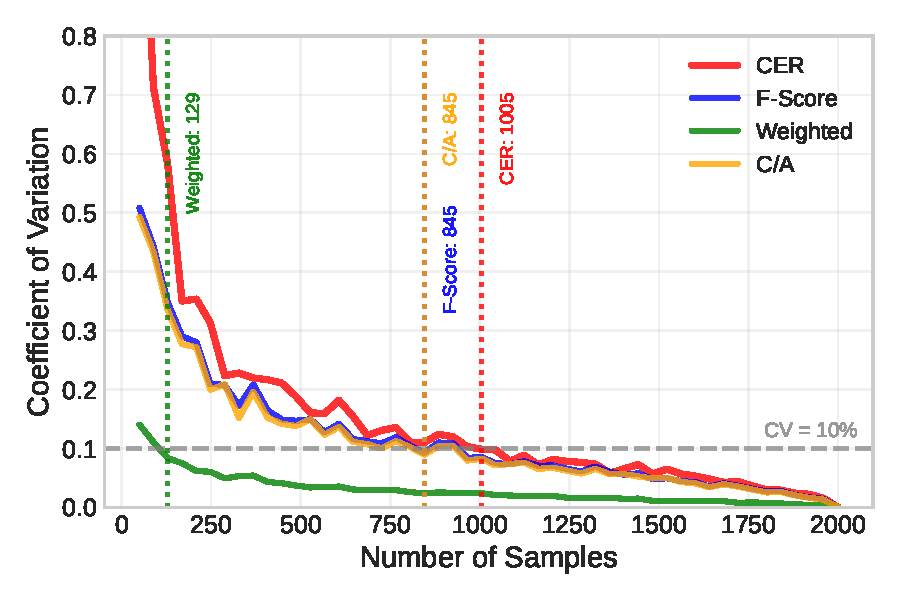
\includegraphics[width=\textwidth]{Figures/cv_comparison.pdf}
        \vspace{0.8em}
        \caption{Coefficient of variation of RI when evaluating on subsets of the full dataset. \cm{Add significance test}}
        \label{fig:refusal_index_cv_subset}
    \end{minipage}
    \hfill
    \begin{minipage}[t]{0.48\textwidth}
        \centering
        \vspace{-18.8em}
        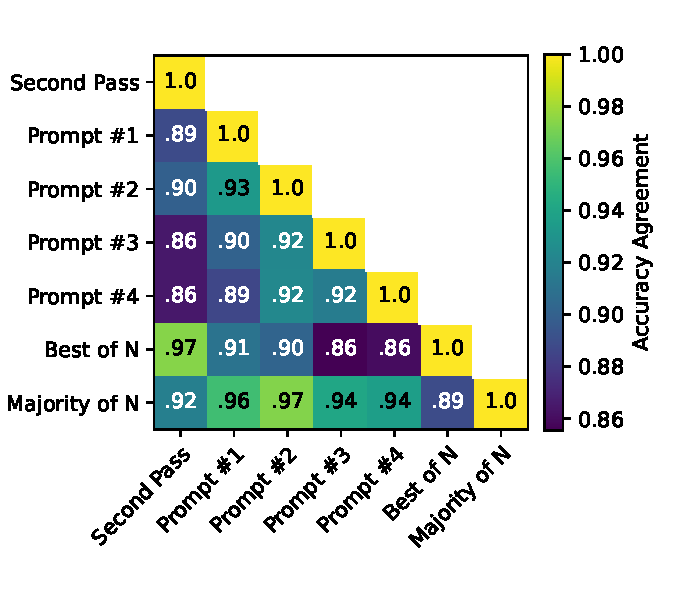
\includegraphics[width=\textwidth]{Figures/prompt_acc_agreement.pdf}
        \caption{Accuracy agreement between different prompt strategies.}
        \label{fig:prompt_acc_agreement}
    \end{minipage}
\end{figure}

We next examine how variations in prompt design affect the RI evaluation. Our experimental setup uses four distinct first-pass prompts, each with different few-shot examples and instructions, to induce varying refusal rates. For the second pass, a single, simpler prompt is used to compel the model to answer all previously refused questions. Although these prompts are designed to produce different refusal rates, it is crucial to verify that they do not introduce confounding effects on model accuracy, which would in turn impact the RI calculation.

To assess this, we measure the accuracy agreement between pairs of prompt strategies. Agreement is calculated as the proportion of questions for which both prompts yielded the same correctness label, considering only the questions answered by both. As shown in Figure~\ref{fig:prompt_acc_agreement}, the accuracy agreement between different first-pass prompts is consistently high (over 90\%). This indicates that the choice of prompt strategy does not significantly alter the model's underlying accuracy on the questions it chooses to answer. Furthermore, the high agreement involving the forced-answer (second-pass) prompt validates its use for effectively estimating the model's baseline accuracy ($\mu$).

\end{document}
